\begin{activity} \label{A:1.1.1}  The following questions concern the position function given by $s(t) = 64 - 16(t-1)^2$, which is the same function considered in Preview Activity \ref{PA:1.1}.
\ba
	\item Compute the average velocity of the ball on each of the following time intervals: $[0.4,0.8]$, $[0.7,0.8]$, $[0.79, 0.8]$, $[0.799,0.8]$, $[0.8,1.2]$, $[0.8,0.9]$, $[0.8,0.81]$, $[0.8,0.801]$.  Include units for each value.
	\item On the provided graph in Figure~\ref{F:1.1.Act1}, sketch the line that passes through the points $A=(0.4, s(0.4))$ and $B=(0.8, s(0.8))$.  What is the meaning of the slope of this line?  In light of this meaning, what is a geometric way to interpret each of the values computed in the preceding question?
	\item Use a graphing utility to plot the graph of $s(t) = 64 - 16(t-1)^2$ on an interval containing the value $t = 0.8$.  Then, zoom in repeatedly on the point $(0.8, s(0.8))$.  What do you observe about how the graph appears as you view it more and more closely?  
	\item What do you conjecture is the velocity of the ball at the instant $t = 0.8$?  Why?
\ea
\begin{figure}[h]
\begin{center}
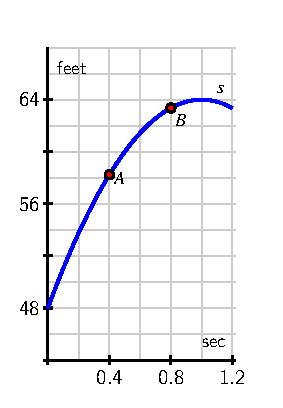
\includegraphics{figures/1_1_Act1.eps}
\caption{A partial plot of $s(t) = 64 - 16(t-1)^2$.} \label{F:1.1.Act1}
\end{center}
\end{figure}
\end{activity}
\begin{smallhint}
\ba
	\item On $[0.4,0.8]$, the average velocity is $AV_{[0.4,0.8]} = \frac{s(0.8)-s(0.4)}{0.8-0.4}$ ft/sec.
	\item Remember that the slope of a line can be found by taking ``rise over run.''  In this context, the slope is found by computing ``change in $s$ over change in $t$.''
	\item While the curve $s(t)$ is a parabola, how does it look up close on a very small interval? 
	\item ``Instantaneous'' velocity can be approximated by average velocity on a very small interval.
\ea
\end{smallhint}
\begin{bighint}
\ba
	\item On $[0.4,0.8]$, the average velocity is $AV_{[0.4,0.8]} = \frac{s(0.8)-s(0.4)}{0.8-0.4}$ ft/sec.  Each of the other average velocities is computed similarly.
	\item Remember that the slope of a line can be found by taking ``rise over run.''  In this context, the slope is found by computing ``change in $s$ over change in $t$.''  Note that each average velocity $\frac{s(b)-s(a)}{b-a}$ can be viewed as the slope of a line between $(a,s(a))$ and $(b,s(b))$.
	\item While the curve $s(t)$ is a parabola, how does it look up close on a very small interval?  What type of familiar function seems to emerge?
	\item ``Instantaneous'' velocity can be approximated by average velocity on a very small interval.  Are the numbers you computed in (a) getting close to a particular value as we look at smaller and smaller intervals surrounding $t = 0.8$?
\ea
\end{bighint}
\begin{activitySolution}
\ba
	\item On $[0.4,0.8]$, the average velocity is $AV_{[0.4,0.8]} = \frac{s(0.8)-s(0.4)}{0.8-0.4} = \frac{63.36-58.24}{0.4} = 12.8$ ft/sec.  On $[0.7,0.8]$, the average velocity is 8 ft/sec.  The other average velocities are, respectively (in the order of the intervals listed in the activity), 6.56, 6.416, 0, 4.8, 6.24, 6.384, all measured in feet per second.
	\item The slope of the line between $A(0.4, s(0.4))$ and $B(0.8, s(0.8))$ is $\frac{s(0.8)-s(0.4)}{0.8-0.4} = 12.8$.  This is precisely the average velocity of the ball between $t = 0.4$ and $t = 0.8$, and indeed each of the average velocities computed in (a) can be viewed as the slope of the line joining the points $(a,s(a))$ and $(b,s(b))$.
	\begin{center}
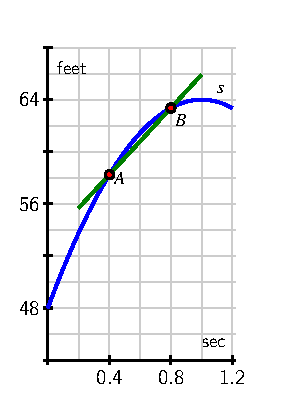
\includegraphics{figures/1_1_Act1Soln.eps}
\end{center}
	\item As we zoom in on the curve $s(t) = 64 - 16(t-1)^2$ at the point $(0.5, 60)$, the graph begins to look like a straight line.  Indeed, it appears to look like a straight line with slope about 6.4.
	\item Observe that the average velocity of the ball on the intervals $[0.799,0.8]$ and $[0.8,0.801]$ is 6.416 and 6.384 feet/sec respectively.  Hence it appears that the ball's velocity at the instant $t = 0.8$ should be about 6.4 feet per second.
\ea
\end{activitySolution}
\aftera